%!TEX root = Nanomat.tex
\ctitle{Struktur og faseoverganger i nanokrystaller}
\paragraph{Oppsummering av kapittelet} Størrelsen og overflatetilstanden til partikler kan påvirke strukturen til materialet; for eksempel har man eksempler på endring i gitterparameter og krystallstruktur. Faseoverganger kan være størrelsesavhengige.\footnote{Advarsel: å lese dette kapittelet, og å prøve å forstå innholdet, er en av de mest frustrerende opplevelsene jeg har hatt i mitt liv. Men det er viktig å huske på at man har både gode og dårlige perioder her i livet, og det kommer bedre tider også, det i kapittel 18 om kolloider er for eksempel ganske lettfattelig og interessant. Poenget er at alt kommer til å gå bra til slutt. Bortsett fra eksamen, da. \emph{Det} kommer til å gå i dass.}

\paragraph{Kornstørrelseavhengighet} Vi har sett at materialer oppfører seg ganske annerledes fra sin makroskopiske form når partiklene blir tilstrekkelig små. I særdeleshet er \idx{korn\-størrelseavhengighet}en til materialene en ny egenskap for nanomaterialer. Vi snakker om to typer bidrag til kornstørrelseavhengigheten:
\begin{itemize}
	\item Andelen overflate- eller grenseflateatomer vokser når kornene blir mindre, slik at overflatens adferd blir mer og mer viktig. Denne typen effekter utvikler seg typisk i form av en monoton funksjon av størrelsen, og lar seg beskrive med termodynamikk.
	\item Hvert korn oppfører seg som en liten boks, og når størrelsen blir liten nok oppstår det nye fenomener inni denne boksen. Denne typen effekter har gjerne å gjøre med elektronstruktur, og er derfor kvantemekaniske av natur. Slike effekter kan ikke nødvendigvis uttrykkes gjennom enkle, monotone funksjoner av størrelsen. Kornene kan ha en bestemt størrelse der effekten er aller størst. 
\end{itemize}

\paragraph{Perovskitter} Bariumtitanat (\ce{BaTiO3}) er hovedeksempelet som kommer til å bli brukt i dette kapittelet.\footnote{Andre materialer av samme type oppfører seg kanskje, men ikke nødvendigvis, som det som beskrives her.} \ce{BaTiO3} tilhører en gruppe artige materialer med \idx{perovskitt}-krystallstruktur, vist i Figur~\ref{fig:perovskite_cell}. Perovskitter har den generelle formen \ce{ABX3} der \ce{A} og \ce{B} begge danner tetragonale gittere (enhetscellene er rektangulære prismer, så man har én gitterkonstant $a$ på den korte siden og en annen gitterkonstant $c$ på langsiden) flettet sammen slik at det er ett \ce{A}-atom i sentrum av hvert \ce{B}-prisme og vice versa. I midten av hver kant i \ce{B}-gitteret (eller ekvivalent, i midten av hver flate i \ce{A}-gitteret) sitter det et \ce{X}-atom (typisk oksygen, da perovskitter typisk er oksider).\footnote{\ce{ABO_{3-$\delta$}} betyr at det er en perovskittstruktur med oksygenvakanser her og der.}\footnote{\ce{LaBaCo2O_{$5+\delta$}} er dobbelperovskitt (skal egentlig være 6 O-er, men det er massevis av vakanser) fordi det kreves en dobbelt så stor enhetscelle for å beskrive materialet. Stod det på tavla en gang. Vet ikke om det er viktig. Håper ikke det.}

\paragraph{Bariumtitanat} Over en temperatur på \SI{120}{\celsius} har \ce{BaTiO3} den ideelle perovskittstrukturen. Hvis temperaturen blir lavere enn dette, oppstår det en asymmetri: hvis man ser på en enhetscelle med \ce{Ti} i sentrum, polariseres materialet ved at \emph{titanionet blir forskjøvet mot ett oksygenion, og vekk fra det andre oksygenionet}, som man ser i Figur~\ref{fig:perovskite_cell}.
\begin{figure}[H]
	\bmd\centering
	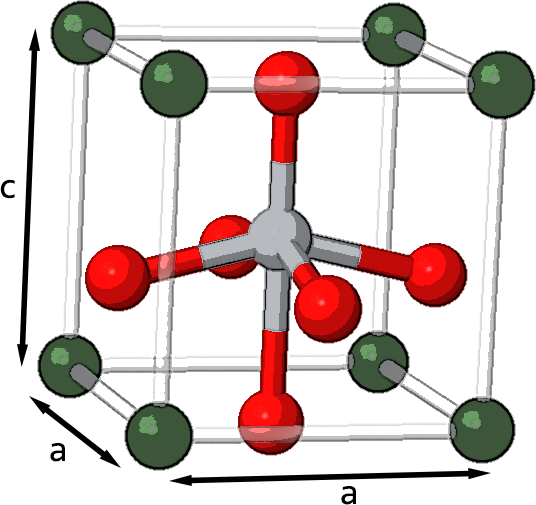
\includegraphics[width=0.9\linewidth]{perovskite.png}
	\caption{Enhetscelle for \ce{BaTiO3} ved $T<\SI{120}{\celsius}$. Grønne atomer er barium, røde atomer er oksygen og det grå atomet er titan.}
	\label{fig:perovskite_cell}
\emd\end{figure}
Denne forskyvningen av \ce{Ti^4+}-kationet gjør enhetscellen til en elektrisk dipol\footnote{Et spørsmål man kan gruble over når man leser dette, er: hvordan bestemmer \ce{Ti^4+} seg for om den skal gå opp eller ned, når situasjonen er helt symmetrisk før overgangen? Svaret er at det er litt sånn tilfeldig, og det vil oppstå domener med forskjellig polarisering, helt analogt med hvordan det oppstår domener med forskjellig magnetisering i ferroelektriske materialer.}. Denne egenskapen gjør \ce{BaTiO3} \emph{ferroelektrisk}\index{ferroelektrisitet} for $T<\SI{120}{\celsius}$. Ferroelektrisitet er når et materiale lagrer energi i form av et permanent elektrisk felt, analogt med hvordan ferromagneter lagrer energi i form av et permanent magnetisk felt. \SI{120}{\celsius} kalles derfor Curie-temperaturen til \ce{BaTiO3}. En relatert effekt som oppstår ved Curie-temperaturen er at den dielektriske konstanten plutselig skyter i været:
\begin{itemize}
	\item $\epsilon_r(\SI{100}{\celsius})\approx 1500$
	\item $\epsilon_r(\SI{120}{\celsius})\approx 11000$
	\item $\epsilon_r(\SI{150}{\celsius})\approx 4000$	
\end{itemize}

\cstitle{Krystallinske faseoverganger i nanokrystaller}
Det finnes flere eksempler på størrelsesbestemte faseoverganger, og innenfor disse eksemplene har vi både keramer, metaller og halvledere. Dette tyder på at \emph{kornstørrelsesavhengige faseoverganger er en iboende egenskap ved alle nanomaterialer}, og ikke begrenset til én bestemt kategori materialer. Eksempler:
\begin{itemize}
	\item \emph{Keramer} (i tillegg til \ce{BaTiO3}): ved romtemperatur og atmosfærisk trykk har vanlig zirkondioksid (\ce{ZrO2}) monoklin krystallstruktur, men over en viss temperatur går krystallstrukturen over til å bli tetragonal. Denne temperaturen er ved ca. \SI{1150}{\celsius} for det makroskopiske materialet, men når krystallene blir mindre enn ca. \SI{40}{\nano\meter} faller plutselig denne overgangstemperaturen dramatisk, og når de er mindre enn ca. \SI{10}{\nano\meter} er det den tetragonale strukturen som er stabil ved romtemperatur.
	\item \emph{Metaller}: smeltepunktene til mange metaller faller når partikkeldiameteren blir mindre. Et eksempel på endring i krystallstruktur er nikkel, som har fcc-struktur i bulk, men endrer til hcp (heksagonal tettpakket struktur) når diameteren er mindre enn \SI{4}{\nano\meter}.
	\item \emph{Halvledere} har ikke blitt studert så nøye som keramer og metaller i denne sammenhengen, men veldig små \ce{CdS}-nanopartikler (diameter på mindre enn \SI{3}{\nano\meter}) kan ha en annen krystallstruktur enn bulkmaterialet.
\end{itemize}

\paragraph{Termodynamikk for nanokrystaller} I en standard termodynamisk behandling av nanokrystaller kan man ta hensyn til kornstørrelseavhengighet ved å legge til et ledd i Gibbs fri energi $G(T,p,N)$ for å få en ny tilstandsfunksjon $G^*(T,p,N,R)$:\footnote{Jeg bruker liten $v$ her, ikke $V$ som i Bréchnigac et. al., fordi det er snakk om molart volum (en intensiv størrelse)}\footnote{Hvorfor $2\gamma v/R$? Svaret er at ikke tenk på det. Et bedre spørsmål er hvorfor vi har et minustegn der. Det betyr jo at den frie energien \emph{minker} når vi \emph{øker} overflatespenningen? What?}
\begin{equation}
	\label{eq:modified_gibbs}
	G^* = G - 2\gamma v / R,
\end{equation}
slik at likevektsbetingelsen blir
\begin{equation}
	\dG^* = 0
\end{equation}
og man har en likevekt mellom to faser $\alpha$ og $\beta$ når
\begin{equation}
	G_{\alpha}^*=G_{\beta}^*.
\end{equation}
For en gitt $(T,p,N)$ vil det da finnes en kritisk radius $R_c$ der faseovergangen skjer. Og for en gitt $(p,N,R)$ vil det finnes en kritisk temperatur $T_c$ der faseovergangen skjer. Eksperimenter på \ce{BaTiO3}-nanopartikler gir resultater som stemmer overens med en slik termodynamisk behandling.\footnote{Så det er jo fint.}

\paragraph{Overflatetilstandens rolle} I de to forrige avsnittene så vi på effekten av å endre kornstørrelsen. Hva om vi holder størrelsen konstant, men endrer overflatetilstanden? Vi kan få til dette ved å la kornene adsorbere kjemikalier, ved å presse sammen nanokornene, eller ved å sette dem inn i et annet fast stoff. 

Fig. 2.7. i Bréchnigac et. al. viser et enkelt eksempel, der vi har kornstørrelse på $x$-aksen, temperatur på $y$-aksen, og de tre kurvene viser hva som skjer når materialet gjennomgår en overgang fra én krystallstruktur til en annen. I den øvre delfiguren er kornene i form av fritt pulver, det vil si at vi har en overgang mellom fast stoff og gass ved overflaten til kornene. I den nedre delfiguren er kornene presset sammen til et agglomerat, slik at vi har en overgang mellom fast stoff og et annet fast stoff ved overflaten til kornene. I den øvre delfiguren har vi, som vi allerede har sett, overgangstemperaturer som er kornstørrelseavhengige. Men når vi presser sammen kornene til et agglomerat forsvinner denne effekten, og overgangstemperaturene er temmelig uavhengig av kornstørrelse. Ikke bare er de temmelig uavhengig av kornstørrelsen - overgangstemperaturene er omtrent de samme som for store korn (altså bulkmaterialet). Dermed ser det ut til at overflateeffekten forsvinner i det polykrystallinske materialet (altså når man har det samme materialet på hver side av en korngrense).

\paragraph{Modifisering av overgangsbarrieren} I nanopartikler kan det, trolig av kinetiske årsaker, oppstå visse eksotiske, metastabile strukturer. For eksempel: i \ce{Ge} (bulkmaterialet) kan man oppnå en viss metastabil fase ved å øke trykket til \SI{10}{\giga\pascal} og raskt senke det til atmosfærisk trykk igjen. Den resulterende strukturen forsvinner hvis materialet så varmes opp til over \SI{200}{\celsius}. I nanopartikler av \ce{Ge} med diameter på mindre enn \SI{4}{\nano\meter} oppstår den samme fasen spontant,\footnote{På grunn av termisk energi, da, antar jeg.} og den forsvinner ikke før man varmer opp til over \SI{800}{\celsius}. Dette tyder på at reduksjon i kornstørrelsen til nanokrystaller medfører at energibarrieren assosiert med denne overgangen synker. Vi kan beskrive dette med den termodynamiske modellen beskrevet av ligning \eqref{eq:modified_gibbs}. Ved en faseovergang er det kun $G$ og $\gamma$ som endrer seg (dersom nanopartiklenes volum og radius antas å være det samme i de to fasene),
\begin{equation}
	\label{eq:particle_delta_g}
	\Delta G^* = \Delta G - \frac{2v}{R}\Delta\gamma,
\end{equation}
så fortegnet til $\Delta \gamma = \gamma_2-\gamma_1$ vil altså bestemme hvordan den modifiserte frie energien påvirkes av partiklenes størrelse. 

\cstitle{Geometriske endringer i nanokrystaller}

\paragraph{Endringer i gittergeometrien} Undersøkelser av \ce{BaTiO3} i nanopulverform viser at selve krystallstrukturen også påvirkes av det finnes en kritisk diameter, $d_C=\SI{80}{\nano\meter}$.\footnote{Bréchnigac bruker $\Phi$ som symbol for diameter, antakelig fordi det ser ut som en sirkel pluss en strek som indikerer diameter. Det blir for dumt. $d$ er fint. Visste du at noen land har dødsstraff for å bruke forvirrende notasjon?} Når $d>d_C$ har \ce{BaTiO3} den vanlige perovskittstrukturen som bulkmaterialet. Etter hvert som diameteren minker blir enhetscellen mer og mer kubisk ($c/a$ går mot $1$, men volumet $a^2c$ til enhetscellen holdes konstant). Når $d<d_C$ antar \ce{BaTiO3} en kubisk perovskittstruktur ($c=a$). Etter hvert som diameteren minker blir $a$ større slik at volumet til enhetscellen øker når partikkelen blir mindre (men merk at akkurat dette trolig har mer å gjøre med varmebehandlingen som brukes for å oppnå denne størrelsen). Med andre ord blir geometrien til krystallstrukturen selv påvirket av kornstørrelsen. Dette er riktignok \emph{ikke} et generelt fenomen - for eksempel finner man ingen lignende effekt i \ce{ZnO}, som også har en avlang krystallstruktur. Man spekulerer i om ikke det kan ha noe å gjøre med at \ce{BaTiO3}-enhetscellen er polar (under Curie-temperaturen), mens \ce{ZnO}-enhetscellen ikke er det.

\paragraph{Endringer i gitterparameteren} For å beskrive hvordan gitterparameteren avhenger av kornstørrelsen, bruker man Laplace' lov,
\begin{equation}
	P_{\text{inne i kornene}}=P_{\text{utenfor kornene}}+4\Gamma/d,
\end{equation}
der $d$ er kornstørrelsen. $\Gamma$ er overflatestress, som er en generalisering av overflatespenning $\gamma$. 

I noen tilfeller, for eksempel for \ce{Co} og \ce{Mn}, kan $\Gamma$ tilnærmes som $\gamma$. Da er det siste leddet positivt og blir større jo mindre kornene blir. Dermed vil det i disse tilfellene bli et økt trykk inne i små korn, slik at atomene presses sammen og gitterparameteren minker.

I andre tilfeller er $\Gamma$ veldig ulik $\gamma$, den kan til og med være negativ. Som du forhåpentligvis har forutsett er dette tilfellet for \ce{BaTiO3}, siden dette materialet som sagt utvider gitteret sitt når partiklene blir små. 

\paragraph{Endrer gitterparameteren seg kontinuerlig når man går fra midten av en nanopartikkel til overflaten av den?} Jepp, ser sånn ut. Er det forresten noen som skjønner figur 2.12? Hva er greia? Hva er det som bestemmer om pilene går innover eller utover?
